\subsection{Aksjomaty przystawania kątów}
Podobnie jak dla odcinków, wprowadzamy niezdefiniowaną relację przystawania kątów, oznaczaną znowu przez $\cong$, ponieważ nie prowadzi to do nieporozumień.

\begin{axiom}[przystawania, C4]
    Dla każdego kąta $\angle BAC$ i każdej $DF$ półprostej istnieje dokładnie jedna półprosta $DE$ po ustalonej stronie prostej $DF$ taka, że $\angle BAC \cong \angle EDF$.
\end{axiom}

Możemy traktować ten aksjomat jako odpowiednik cyrkla: pozwala przenosić kąty tak, jak Euklides (I.23).

\begin{axiom}[przystawania, C5]
    Niech $\alpha, \beta, \gamma$ będą kątami.
    Jeśli $\alpha \cong \beta$ oraz $\alpha \cong \gamma$, to $\beta \cong \gamma$.
    Każdy kąt przystaje do siebie: $\alpha \cong \alpha$.
\end{axiom}

Mamy wreszcie cechę przystawania bok-kąt-bok, z której można wyprowadzić dodawanie kątów:

\begin{axiom}[przystawania, C6]
    Niech $ABC$ i $DEF$ będą dwoma trójkątami takimi, że $AB \cong DE$, $AC \cong DF$ i $\angle BAC \cong \angle EDF$.
    Wtedy pozostałe boki i kąty są przystające, a razem z nimi całe trójkąty: $BC \cong EF$, $\angle ABC \cong \angle DEF$ i $\angle ACB \cong \angle DFE$.
\end{axiom}

Euklides udawał, że dowodzi aksjomatu C6 metodą ,,nakładania'' figur, ale Hilbert znalazł model będący świadkiem, że nie wynika on z poprzednich aksjomatów; patrz \cite[paragraf 11]{hilbert_1988}, jak wiemy od Greenberga \cite[s. 200]{greenberg_2010}.

Jeżeli chodzi o dodawanie kątów, musimy być ostrożni.
Suma dwóch kątów może okazać się prostą (lub ,,dwoma kątami prostymi'' jak pisze Euklides) albo mieć miarę większą niż $\pi$, wtedy składniki sumy nie znajdują się we wnętrzu otrzymanego kąta.
Kąty można także odejmować.

\begin{definition}[kąt przyległy]
    Niech $\angle BAC$ będzie kątem, zaś $D$ punktem na prostej $AC$ po przeciwnej stronie $A$ niż $C$.
    Wtedy kąty $\angle BAC$ i $\angle BAD$ nazywamy przyległymi. % supplementary.
\end{definition}

Warto teraz spojrzeć na (I.13) Euklidesa.


\begin{figure}[H] \centering
\begin{tikzpicture}[scale=.6]
    \tkzDefPoint(-4, -2){A}
    \tkzDefPoint(4, 2){B}
    \tkzDefPoint(4, -2){C}
    \tkzDefPoint(-4, 2){D}
    \tkzDefPoint(0, 0){Zero}
    \tkzDefPoint(0, 0.7){X1}
    \tkzDefPoint(-1.7, 0){X2}
    \tkzDefPoint(1.7, 0){X3}
    \tkzMarkAngle[arc=l,size=1.2,mark=||](D,Zero,A)
    \tkzMarkAngle[arc=l,size=1.2,mark=||](C,Zero,B)
    \tkzMarkAngle[arc=ll,size=1.2](B,Zero,D)

    \tkzDrawSegments[line width=0.3mm](A,B)
    \tkzDrawSegments[line width=0.3mm](C,D)
    \tkzLabelPoint[anchor=center](X1){$\beta$}
    \tkzLabelPoint[anchor=center](X2){$\alpha$}
    \tkzLabelPoint[anchor=center](X3){$\gamma$}

\end{tikzpicture}
    \caption{kąty przyległe ($\alpha$ i $\beta$) oraz wierzchłkowe ($\alpha$ i $\gamma$)}
\end{figure}

\begin{proposition}
    Kąty wierzchołkowe (para kątów przy dwóch przecinających się prostych, które nie są przyległe) są przystające.
\end{proposition}

% odpowiadające i naprzemianległe.
\todofoot{Pompe s. 5: dwie proste przecięte trzecią wyznaczają kąty tej samej miary <=> proste są równoległe (naprzemianległe). Pompe s. 5: suma kątów trójkąta to 180}

Istnieje odpowiednik relacji między odcinkami ,,bycia mniejszym'' dla kątów:

\begin{definition}
    Niech $\angle BAC$ i $\angle EDF$ będą kątami.
    Jeśli istnieje półprosta $DG$ wewnątrz kąta $EDF$ taka, że $\angle BAC \cong \angle GDF$, to powiemy, że kąt $\angle BAC$ jest mniejszy niż kąt $\angle EDF$ (a ten drugi jest większy niż pierwszy).
\end{definition}

\begin{definition}
    Kąt, który przystaje do kąta przyległego, nazywamy prostym.
    Dwie proste, które przecinają się i wyznaczają tam cztery kąty proste, będziemy nazywać prostopadłymi.
\end{definition}

Nie jest ważne, który kąt przyległy wybierzemy, ponieważ kąty wierzchołkowe są przystające.
